\section{Data}

The same datasets are used as in Reed et al. \cite{reed2016learning}, namely, Caltech-UCSD \textit{birds} 200 \cite{welinder2010caltech} and Oxford-102 \textit{flowers} \cite{Nilsback08}. The former contains nearly 12 thousand photos scraped from Flickr of 200 bird species. As can be seen in Figure \ref{fig:birds_histogram}, each class contains at most 60 images, and is quite balanced. The Oxford flowers dataset is similar in nature but focuses on common species of flowers from around the United Kingdom. It is less balanced (see Figure \ref{fig:flowers_histogram}) and also contains slightly fewer, about 8 thousand images. Nonetheless, in practice, \textit{birds} is reported to be more challenging for learning \cite{reed2016learning,reed2016generative}.

Next to their class label, each image also comes with 10 short descriptions crowdsourced by Reed et al. \cite{reed2016learning}. These only focus on the subject of the photos and are rich in feature descriptions. Thus, overall there are about 100k \texttt{(image, caption, species)} datapoints for training and evaluation.

\begin{figure}
  \centering
  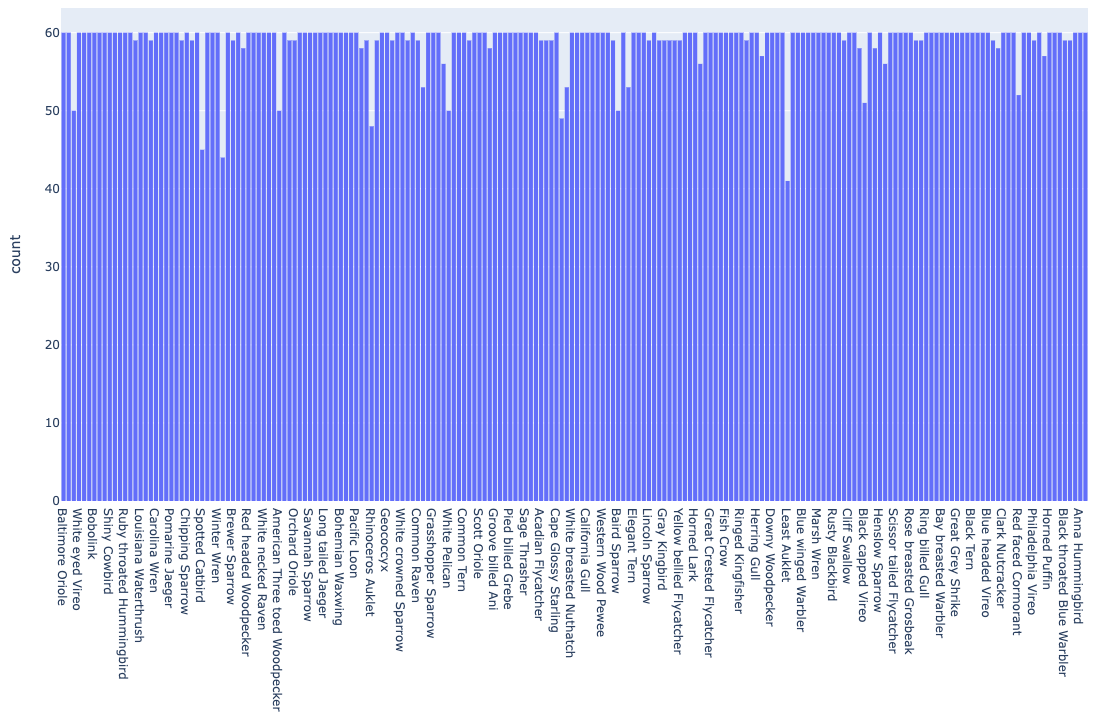
\includegraphics[width=1 \linewidth]{figures/bird_classes.png}
  \caption{Distribution of classes (species) in the Caltech-UCSD birds 200 dataset \cite{welinder2010caltech}.}
  \label{fig:birds_histogram}
\end{figure}

\begin{figure}
  \centering
  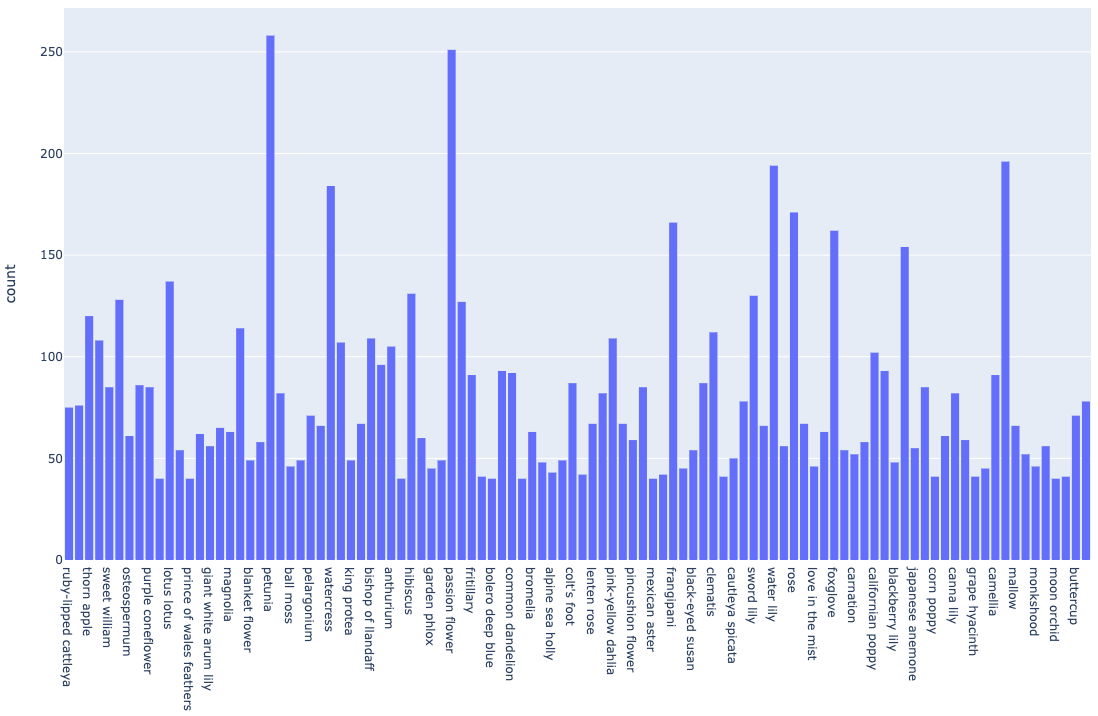
\includegraphics[width=1 \linewidth]{figures/flower_classes.png}
  \caption{Distribution of classes (species) in the Oxford-102 flowers dataset \cite{Nilsback08}.}
  \label{fig:flowers_histogram}
\end{figure}

The datasets were selected for their fine-grained nature. For example, discriminating automobiles from trees is less challenging than telling apart trees of different species. Especially in the case of \textit{birds}, this is further complicated by the dissimilar visual appearance of males and females of the same species. Additionally, both \textit{birds} and \textit{flowers} are a product of nature, resulting in large relative variance even between the instances of the same class. Hence, these can serve as an ideal testbed for investigating how models pretrained on more general classes can be fine-tuned for subtle ones.
